% !TEX program = pdflatex
% !TEX options = -synctex=1 -interaction=nonstopmode -file-line-error "%DOC%"
% 固体物理第十一次作业
\documentclass[UTF8,10pt,a4paper]{article}
\usepackage{ctex}
% \catcode`\。=\active
% \newcommand{。}{.}
\newcommand{\CourseName}{固体物理}
\newcommand{\CourseCode}{PHYS1502}
\newcommand{\Semester}{2019-2020学年第二学期}
\newcommand{\ProjectName}{第十一次作业}
\newcommand{\DueTimeType}{截止时间}
\newcommand{\DueTime}{2020. 5. 22(周五)17:00}
\newcommand{\StudentName}{陈稼霖}
\newcommand{\StudentID}{45875852}
\usepackage[vmargin=1in,hmargin=.5in]{geometry}
\usepackage{fancyhdr}
\usepackage{lastpage}
\usepackage{calc}
\pagestyle{fancy}
\fancyhf{}
\fancyhead[L]{\CourseName}
\fancyhead[C]{\ProjectName}
\fancyhead[R]{\StudentName}
\fancyfoot[R]{\thepage\ / \pageref{LastPage}}
\setlength\headheight{12pt}
\fancypagestyle{FirstPageStyle}{
    \fancyhf{}
    \fancyhead[L]{\CourseName\\
        \CourseCode\\
        \Semester}
    \fancyhead[C]{{\Huge\bfseries\ProjectName}\\
        \DueTimeType\ : \DueTime}
    \fancyhead[R]{姓名 : \makebox[\widthof{\StudentID}][s]{\StudentName}\\
        学号 : \StudentID\\
        成绩 : \underline{\makebox[\widthof{\StudentID}]{}}}
    \fancyfoot[R]{\thepage\ / \pageref{LastPage}}
    \setlength\headheight{36pt}
}
\usepackage{amsmath,amssymb,amsthm,bm}
\allowdisplaybreaks[4]
\newtheoremstyle{Problem}
{}
{}
{}
{}
{\bfseries}
{.}
{ }
{第\thmnumber{ #2}\thmname{ #1}\thmnote{ (#3)} 得分: \underline{\qquad\qquad}}
\theoremstyle{Problem}
\newtheorem{prob}{题}
\newtheoremstyle{Solution}
{}
{}
{}
{}
{\bfseries}
{:}
{ }
{\thmname{#1}}
\makeatletter
\def\@endtheorem{\qed\endtrivlist\@endpefalse}
\makeatother
\theoremstyle{Solution}
\newtheorem*{sol}{解}
\providecommand{\abs}[1]{\left\lvert#1\right\rvert}
\usepackage{graphicx}
\usepackage{subfigure}
\usepackage{listings}
\begin{document}
\thispagestyle{FirstPageStyle}
\begin{prob}[(16.1) Metal and Insulators]
    Explain the following:
    \begin{enumerate}
        \item[(a)] sodium, which has two atoms in a bcc (conventional cubic) unit cell, is a metal;
        \item[(b)] calcium, which has four atoms in a fcc (conventional cubic) unit cell is a metal;
        \item[(c)] diamond, which has eight atoms in a fcc (conventional cubic) unit cell with a basis, is an electrical insulator, whereas silicon and germanium, which have similar structures, are semiconductors. (Try to think up several possible reasons!)
        \begin{itemize}
            \item[$\triangleright$] Why is diamond transparent?
        \end{itemize}
    \end{enumerate}
\end{prob}
\begin{sol}
    \begin{enumerate}
        \item[(a)] 钠的原胞中只含有一个原子,每个原子提供一个电子,导致半满的能带,因此是导体.
        \item[(b)] 钙的原胞中也只含有一个原子,每个原子提供两个电子,但是由于其晶格产生的周期性势场不是很强,没有产生(很大的)带隙,所以即使是价带被填满,价带的电子依然可以在外场的作用下轻易地到导带上去,产生电流,因此也是导体.
        \item[(c)] 金刚石、硅、锗的原胞中都含有两个原子,每个原子有四个价电子(s轨道贡献两个电子,p轨道贡献两个电子),因此下面的四条价带被完全填满,上面的四条导带空着. 在这三种材料中,金刚石的原子体积小,所以离价电子的距离近,晶格的周期势场对电子波函数的影响就强,所以打开的带隙更大($5.47$eV),是绝缘体,而硅和锗的带隙相对就较小(硅的带隙为$1.12$eV,锗的带隙为$0.66$eV),为半导体.\\
        另一种解释:对于C,基态下电子填充到的最高轨道为2p轨道,它与能量稍高的3s轨道的能量差较大,因此组成晶体后,电子依然主要束缚在3s轨道上;而对于Si和Ge,基态下电子填充到的最高轨道为3p和4p,与能量稍高的轨道之间的差距并不那么大,所以电子更容易激发到稍高的轨道上去,也就是有更小的带隙.
        \begin{itemize}
            \item[$\triangleright$] 由于金刚石的带隙很大,所以可见光无法将价带上的电子激发到导带上去,故金刚石很难吸收可见光,呈透明状.
        \end{itemize}
    \end{enumerate}
\end{sol}

\begin{prob}[(16.2) Fermi Surface Shapes]
    \begin{enumerate}
        \item[(a)] Consider a tight binding model of atoms on a (two-dimensional) square lattice where each atom has a single atomic orbital. If these atoms are monovalent, describe the shape of the Fermi surface.
        \item[(b)] Now suppose the lattice is not square, but is rectangular instead with primitive lattice vector of length $a_x$ and $a_y$ in the $x$ and $y$ directions respectively, where $a_x>a_y$. In this case, imagine that the hopping have a value $-t_x$ in the $x$-direction and a value $-t_y$ in the $y$-direction, with $t_y>t_x$. (Why does this inequality match $a_x>a_y$?)
        \begin{itemize}
            \item[$\triangleright$] Write an expression for the dispersion of the electronic states $\epsilon(\bm{k})$.
            \item[$\triangleright$] Suppose again that the atoms are monovalent, what is the shape of the Fermi surface now?
        \end{itemize}
    \end{enumerate}
\end{prob}
\begin{sol}
    \begin{enumerate}
        \item[(a)] 电子的状态可表为
        \begin{align}
            \lvert\Psi\rangle=\sum_{n_x,n_y}\phi_{n_x,n_y}\lvert n_x,n_y\rangle.
        \end{align}
        其中$\lvert n_x,n_y\rangle$代表电子处在各个原子上的状态.
        电子在二维晶体中的总哈密顿为
        \begin{align}
            \hat{H}=\hat{H}_0+\hat{V}_h.
        \end{align}
        其中$H_0$为电子处在某个独立电子上的哈密顿,$V_h$为hopping能. 总哈密顿在$\{\lvert n_x,n_y\rangle\}$表象中的矩阵元为
        \begin{align}
            H_{m_xm_y,n_xn_y}=\langle m_x,m_y\lvert\hat{H}\rvert n_x,n_y\rangle=\langle m_x,m_y\rvert\hat{H}_0\lvert n_x,n_y\rangle+\langle m_x,m_y\rvert\hat{V}_h\lvert n_x,n_y\rangle,
        \end{align}
        其中
        \begin{align}
            \langle m_x,m_y\rvert\hat{H}_0\lvert n_x,n_y\rangle=&\varepsilon_0\delta_{m_xn_x}\delta_{m_yn_y},\\
            \langle m_x,m_y\rvert\hat{V}_h\lvert m_x,m_y\rangle=&\left\{\begin{array}{ll}
                -t,&(m_x=n_x\pm 1,m_y=n_y\pm 1)\text{ 或 }(m_x=n_x,m_y=n_y\pm 1),\\
                0,&\text{otherwise}.
            \end{array}\right.
        \end{align}
        (假设只有最近的两个原子之间才存在hopping)\\
        电子的薛定谔方程为
        \begin{align}
            \hat{H}\lvert\Psi\rangle=E\lvert\Psi\rangle,
        \end{align}
        其分量形式为
        \begin{align}
            -t\phi_{n_x-1,n_y}-t\phi_{n_x,n_y-1}+\varepsilon_0\phi_{n_x,n_y}-t\phi_{n_x+1,n_y}-t\phi_{n_x,n_y+1}=E\phi_{n_x,n_y}.
        \end{align}
        利用周期性边界条件,设解为
        \begin{align}
            \phi_{n_x,n_y}=Ae^{ik_xn_ya+ik_yn_ya}.
        \end{align}
        将猜测的解代入薛定谔方程中,得色散关系
        \begin{align}
            E(\bm{k})=\varepsilon_0-2t[\cos(k_xa)+\cos(k_ya)].
        \end{align}
        绘制其等高线图如图\ref{2-E-k-square}.
        \begin{figure}[h]
            \centering
            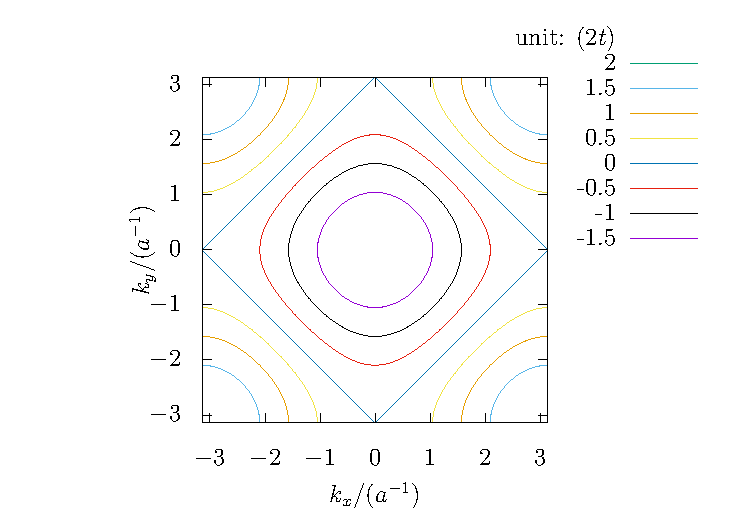
\includegraphics[width=.6\textwidth]{2-E-k-square.pdf}
            \caption{二维方格子的色散关系等高线图.}
            \label{2-E-k-square}
        \end{figure}
        \\由于每个原子贡献一个价电子,所以二维方格子的能带是半满的,其费米面即图中蓝色实线围成的区域,为一个正方形.
        \item[(b)] $a_x>a_y$ 对应 $t_y>t_x$,这是因为晶格常数(原子间距)越大,电子在原子之间的跃迁就越弱.
        \begin{itemize}
            \item[$\triangleright$] 对于$a_x>a_y$,$t_y>t_x$的矩形格子,其hopping能算符的矩阵元为
            \begin{align}
                \langle m_x,m_y\rvert\hat{V}_h\lvert n_x,n_y\rangle=\left\{\begin{array}{ll}
                    -t_x,&m_x=n_x\pm 1,m_y=n_y,\\
                    -t_y,&m_x=n_x,m_y=n_y\pm 1,\\
                    0,&\text{otherwise}.
                \end{array}\right.
            \end{align}
            故电子的薛定谔方程的分量形式为
            \begin{align}
                -t_x\phi_{n_x-1,n_y}-t_y\phi_{n_x,n_y-1}+\varepsilon_0-t_x\phi_{n_x+1,n_y}-t_y\phi_{n_x,n_y+1}=E\phi_{n_x,n_y}.
            \end{align}
            利用周期性边界条件,设解为
            \begin{align}
                \phi_{n_x,n_y}=Ae^{ik_xn_xa_x+ik_yn_ya_y}.
            \end{align}
            将猜测的解代入薛定谔方程中,得色散关系
            \begin{align}
                E(\bm{k})=\varepsilon_0-2[t_x\cos(k_xa_x)+t_y\cos(k_ya_y)].
            \end{align}
            \item[$\triangleright$] 设$a_x=2a_y=a$,$2t_x=t_y=t$,绘制色散关系登高线图如图\ref{2-E-k-rectangular}.
            \begin{figure}[h]
                \centering
                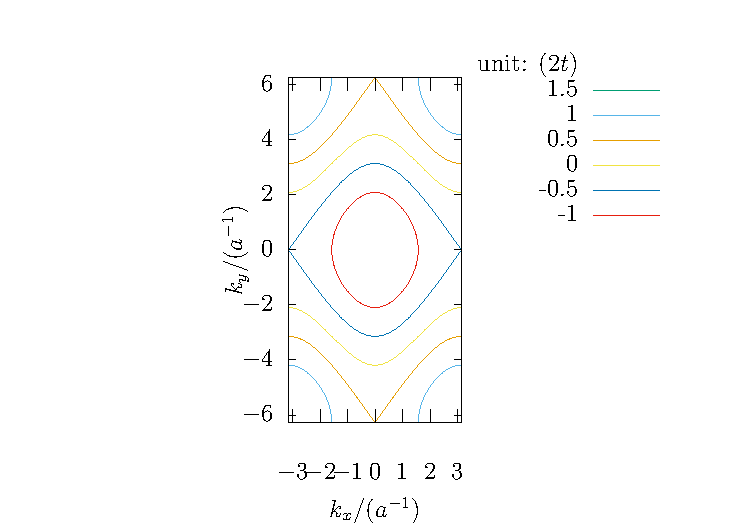
\includegraphics[width=.6\textwidth]{2-E-k-rectangular.pdf}
                \caption{二维矩形格子的色散关系登高线图.}
                \label{2-E-k-rectangular}
            \end{figure}
            \\此时费米面即为图中淡黄色曲线所围区域,相对于二维方格子的费米面已经发生了形变.
        \end{itemize}
    \end{enumerate}
\end{sol}

\begin{prob}[补充问题]
    二维平面上的自由电子受到一个正方形晶格的散射。该晶格的晶格常数为$0.25$ nm。请利用近自由电子近似理论和Matlab程序,画出不同晶格势强度下第一布里渊区中能量最低的两条能带(就像课堂上展示的那种三维图)。并画出沿着某些高对称线上的能带(就像教材图13.7展示的那种二维图)。通过调节晶格势强度,展示出能带从没有带隙到打开带隙的过程。要注意当晶格势比较弱的时候,第二条能带的最低点比第一条能带的最高点还要低,这种体系被称为“半金属”。要在计算结果中展现出这一现象来。
\end{prob}
\begin{sol}
    二维正方形晶格的倒格子的基矢长度为
    \begin{align}
        \abs{G}=\frac{2\pi}{a}=8\pi\text{nm}^{-1}.
    \end{align}
    故第一布里渊区的范围为$[-4\pi\text{nm}^{-1},4\pi\text{nm}^{-1}]$.
    电子的哈密顿量可表为
    \begin{align}
        \hat{H}=\left(\begin{matrix}
            E_1&V_G\\
            V_G^*&E_2
        \end{matrix}\right).
    \end{align}
    其中$E_1=\frac{\hbar^2}{2m}(k_x^2+k_y^2)$是简约布里渊区中的较低的那一支能带能量,$E_2$是简约布里渊区中的较高的那一支能带能量.
    解得本征能量为
    \begin{align}
        E=\frac{(E_1+E_2)^2+\sqrt{(E_1+E_2)^2+V_G^2}}{2}.
    \end{align}
    从$0$(即自由电子)逐渐增大$V_G$,绘制出三维的能带和沿着高对称线的能带如组图\ref{3-E-k}(最后一页).
    \newpage
    \begin{figure}[h]
        \centering
        \subfigure[$V_G=0$,三维能带图]{
        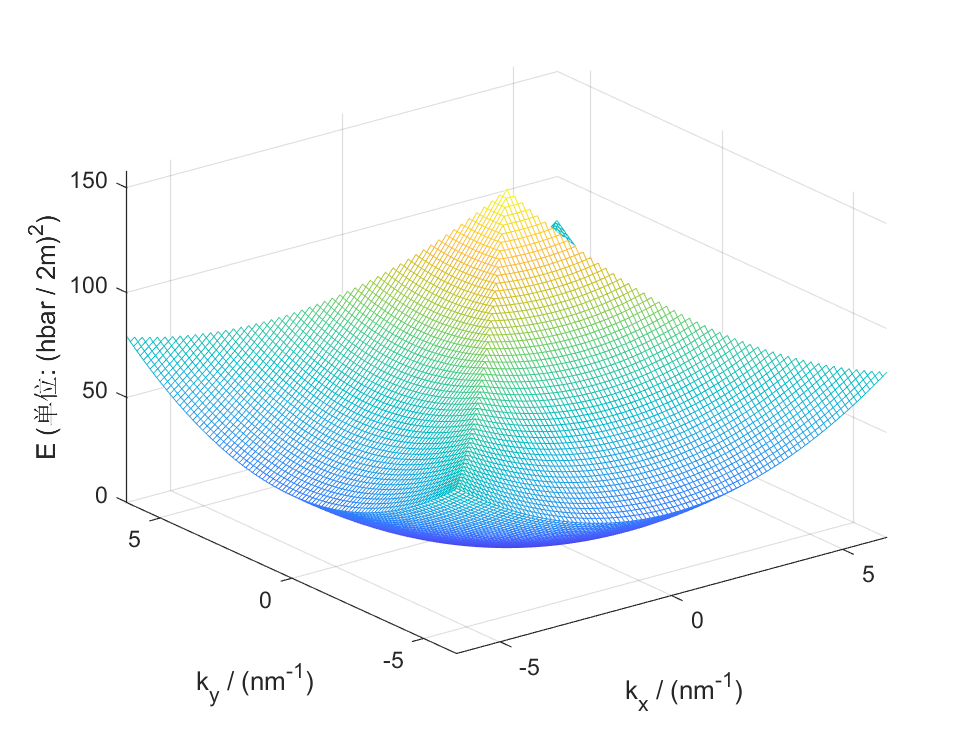
\includegraphics[width=.40\textwidth]{3-E-k-3d-0.png}}
        \subfigure[$V_G=0$,沿着高对称线的能带图]{
        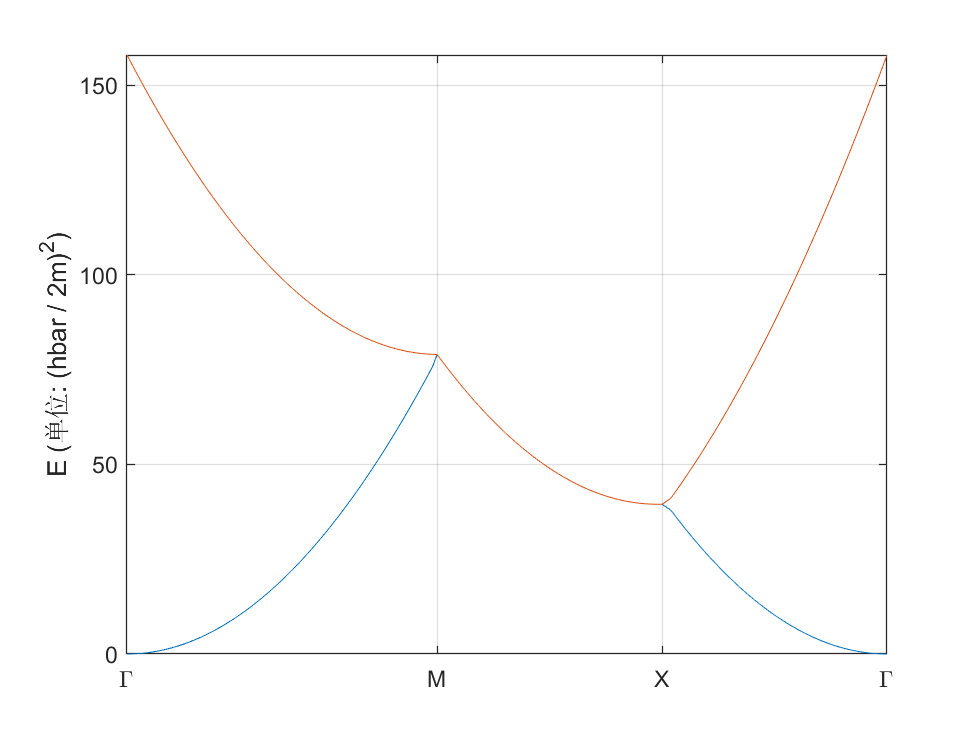
\includegraphics[width=0.45\textwidth]{3-E-k-2d-0.png}}
        \subfigure[$V_G=20$,三维能带图]{
        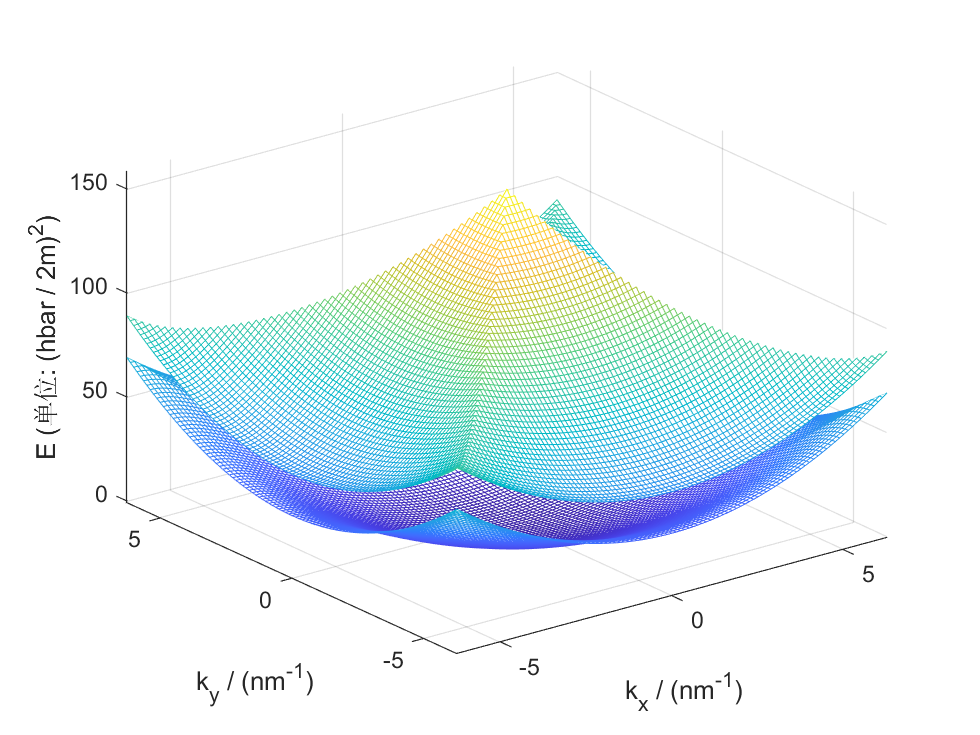
\includegraphics[width=.40\textwidth]{3-E-k-3d-20.png}}
        \subfigure[$V_G=20$,沿着高对称线的能带图]{
        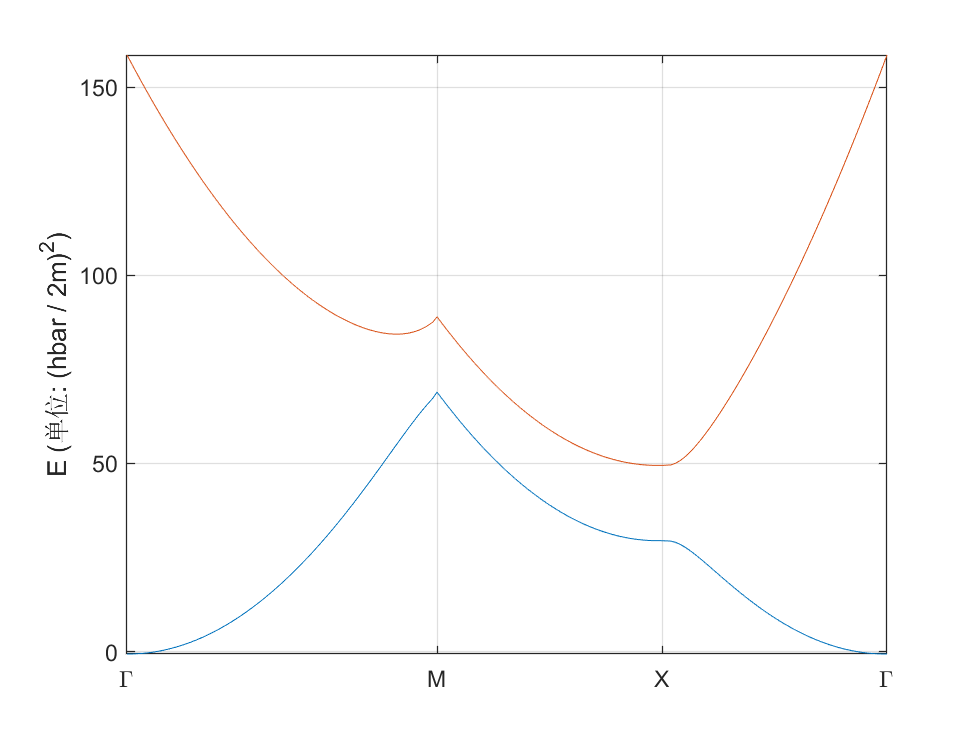
\includegraphics[width=0.45\textwidth]{3-E-k-2d-20.png}}
        \subfigure[$V_G=50$,三维能带图]{
        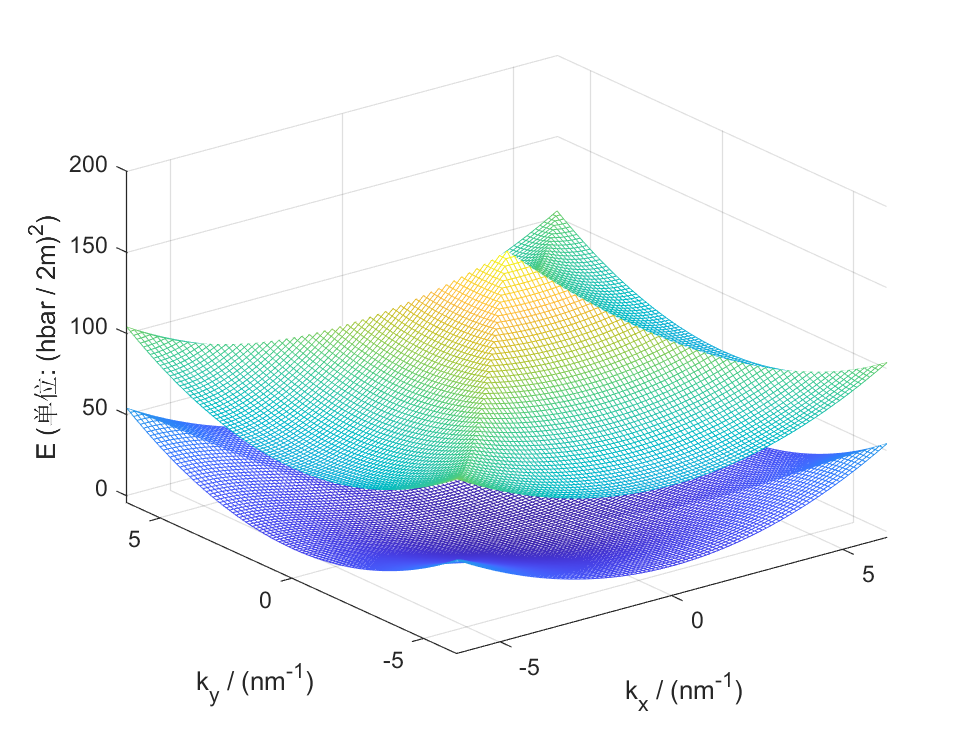
\includegraphics[width=.40\textwidth]{3-E-k-3d-50.png}}
        \subfigure[$V_G=50$,沿着高对称线的能带图]{
        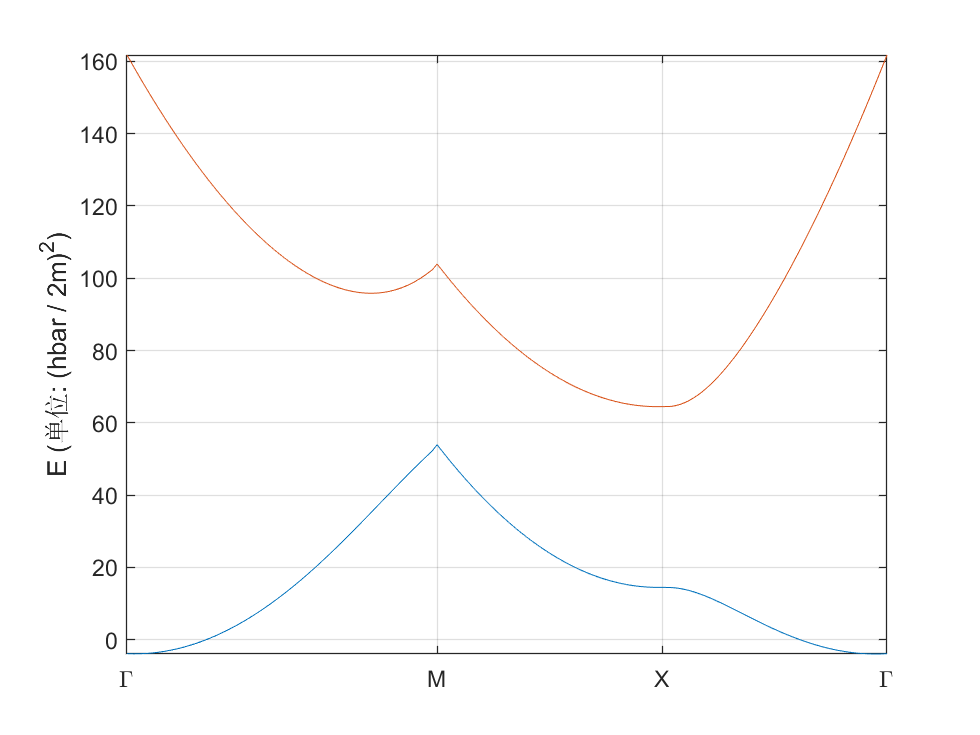
\includegraphics[width=0.45\textwidth]{3-E-k-2d-50.png}}
        \caption{带隙随$V_G$增大逐渐打开的过程.}
        \label{3-E-k}
    \end{figure}

    组图中第一行,无微扰,$V_G=0$,对应了自由电子的能带结构,此时不存在带隙;组图中第二行,当稍增大$V_G$,此时由于晶格周期性势场的围绕,带隙被稍稍打开,但此时第二条能带的最低点比第一条能带的最高点更低,是为半金属;组图中第二行,继续增大$V_G$,带隙变得足够大,此时第二条能带完全在第一条能带以上,存在简介带隙,因此为绝缘体.

    代码如下,在老师提供的代码的基础上进行了部分修改.
\begin{lstlisting}
figure(1)
G = 4 * pi;
[kx,ky] = meshgrid(-G / 2:G / 100:G / 2);
E1 = kx.^2 + ky.^2;
for i = 1:1:101
    for j = 1:1:101
        if ky(i,j) < kx(i,j)
            if ky(i,j) < -kx(i,j)
                E2(i,j) = kx(i,j)^2 + (ky(i,j) + G)^2;
            else
                E2(i,j) = (kx(i,j) - G)^2 + ky(i,j)^2;
            end
        else
            if ky(i,j) < -kx(i,j)
                E2(i,j) = (kx(i,j) + G)^2 + ky(i,j)^2;
            else
                E2(i,j) = kx(i,j)^2 + (ky(i,j) - G)^2;
            end
        end
    end
end
% mesh(kx,ky,E1)
% hold on
% mesh(kx,ky,E2)

VG = 0;
E1_perturbed = ((E1 + E2) - sqrt((E1 - E2).^2 + VG^2)) / 2;
E2_perturbed = ((E1 + E2) + sqrt((E1 - E2).^2 + VG^2)) / 2;
mesh(kx,ky,E1_perturbed)
hold on
mesh(kx,ky,E2_perturbed)
xlabel('k_x / (nm^{-1})','interpreter','tex')
ylabel('k_y / (nm^{-1})','interpreter','tex')
zlabel('E (unit: (hbar / 2m)^2)')

figure(2)
for i = 1:1:51
    k(i) = sqrt(2) * G / 100 * i;
    E3(i) = E1_perturbed(50 + i,50 + i);
    E4(i) = E2_perturbed(50 + i,50 + i);
end
for i = 1:1:51
    k(50 + i) = k(50) + G / 100 * i;
    E3(50 + i) = E1_perturbed(101,102 - i);
    E4(50 + i) = E2_perturbed(101,102 - i);
end
for i = 1:1:51
    k(100 + i) = k(101) + G / 100 * i;
    E3(100 + i) = E1_perturbed(102 - i,51);
    E4(100 + i) = E2_perturbed(102 - i,51);
end
plot(k,E3)
hold on
plot(k,E4)
grid on
xlim([k(1),k(end)])
ylim([min(E3),max(E4)])
xticks([k(1) k(51) k(101) k(151)])
xticklabels({'\Gamma','M','X','\Gamma'})
ylabel('E (unit: (hbar / 2m)^2)')
\end{lstlisting}
\end{sol}
\end{document}